\documentclass[journal,onecolumn,10pt]{IEEEtran}
\usepackage{amsmath,graphicx,url}
\begin{document}
\title{How Much Recalibration Is Enough? Reliability of Cellular Throughput Forecasts Across Networks with Missing Radio Telemetry}
\author{Md. Moazzem Hossain Majumder}
\maketitle
\begin{abstract}
We study whether a small chronological prefix of labeled sessions can calibrate a lower forecast of downlink throughput in two commercial measurement campaigns in Rome. The source-calibrated forecaster exceeds a nominal ten percent violation rate in all four held-out evaluations. At ten target labels the global correction meets the empirical target in each regime, but its supported fraction ranges from 0.006 to 0.073. Missingness-group calibration gives the same results at that budget. Replacing throughput-reset segments with segments beginning at active transitions substantially changes the endpoint distribution and measured violations. On a separate Irish next-row benchmark, calibrated persistence raised supported throughput from 55.60 to 59.44 percent with mean violations of 9.71 percent. Under joint campaign and operator shift in Rome, persistence violated 20.39 percent of forecasts. A clock-triggered replay on that operator supported 16.00 percent with 13.82 percent violations. On two held-out Norwegian bus-route dates a locally fitted tree supported 30.60 percent with 1.02 percent violations. On chronologically held-out Irish dates, ten-label persistence had 34.81 percent violations. The differing endpoints and sparse collection dates limit deployment inference.
\end{abstract}
\begin{IEEEkeywords}
Cellular throughput, conformal prediction, measurement methodology, missing radio telemetry.
\end{IEEEkeywords}

\section{Question and related work}
An application that chooses a sending rate before a download needs to know how often its forecast exceeds delivered throughput and how much usable rate it gives up to reduce those violations. We ask how those quantities change when an operator has only a few labeled examples from the destination network. The contribution is an empirical comparison on released traces, with a common predictor and a fixed test suffix across label budgets. Prior work characterizes the underlying campaigns \cite{kousias2024large,caso2024chronicles}, additive prediction with missing observations \cite{jacobson2025predicting}, and conditional calibration under missing covariates \cite{zaffran2023conformal}. The BAMMO-inspired baseline uses our pattern-specific boosted trees. We did not replicate the original authors' implementation. Grouping by recorded telemetry availability gives a simple comparator. Its interpretation depends on support within each group.

Our contributions are (i) a chronological label-budget benchmark reporting both violations and supported rate, (ii) a controlled comparison of session endpoints with a clock-triggered replay, and (iii) a published Irish benchmark reproduction and a separate evaluation of the ten-label rule on Norwegian measurements. The empirical question is how these choices affect the rate an application could commit under the stated offline decision rule.
Narayanan et al.\ mapped and predicted commercial millimeter-wave throughput \cite{narayanan2020lumos5g}, while Kousias et al.\ modeled performance in non-standalone networks \cite{kousias2024empirical}. Our benchmark evaluates how much measured rate remains supportable when an existing point forecast receives only a short destination calibration prefix.
\section{Measurements and prediction time}
The earlier campaign uses the active throughput CSV in Zenodo 8224890. We take the last available mean download throughput at a DQA completion marker within a campaign and convert kb/s to Mbps. In the later active archive (Zenodo 14073311), we use 43 Ookla traces and process each operator's nonnegative numeric mean-download series separately, converting its documented column units to Mbps. With reset segmentation the releases yield 1,132 operational sessions and 1,001 eligible forecast pairs across development and evaluation. The main evaluation uses only held-out suffixes.
Each forecast uses the preceding result, elapsed time since that segment ended, its duration, recent radio measurements and availability indicators, and scenario. Among the 1,001 eligible pairs, 585 have only LTE measurements and 416 have both LTE and NR. No eligible pair lacks LTE. Consequently, grouping by NR presence and grouping by the two radio indicators define the same partition in this sample. In the later archive, the first throughput reading triggering a reset identifies the prediction time retrospectively. An online deployment would need an independent test-start signal. Even when predictors exclude that reading, selecting forecast times from the outcome trajectory can change the evaluated population. The primary protocol allows up to 60 seconds of lag age. Missing indicators describe what the logger observed. A missing NR signal by itself cannot identify a particular network state or its cause. Lagged throughput requires feedback from completed tests throughout evaluation. A budget of zero refers only to target labels used to fit the calibration offset.

E0 uses five successive blocks of earlier Op1 collection days for training, validation, source calibration, target prefixes and testing. The first three blocks contribute 57, 9 and 33 observations. The benchmark freezes that predictor and source offset for all four regimes. E1 moves to later Op1, E2 to earlier Op2 and E3 to later Op2. Transfer calibration and test blocks use the first approximately 40 percent and last approximately 60 percent of target days, respectively, with integer day boundaries. We take the first $K$ eligible sessions in timestamp order from the calibration pool. E0 has ten available, so its fifteen-session comparison is unavailable. Cross-operator analysis on contemporaneous campaigns is retrospective.

\section{Calibration and metrics}
Let $f$ denote the frozen histogram gradient boosting model and $y$ the endpoint throughput. Split calibration orders the signed scores $f(x_i)-y_i$. For $n$ finite scores, take rank $r=\lceil(n+1)(1-\alpha)\rceil$ in ascending order. When $r>n$ we use positive infinity. The lower forecast is $L=\max(0,f(x)-q)$. A tie at the bound counts as covered. Since $r\le n$ is equivalent to $(n+1)(1-\alpha)\le n$, finite scores yield a finite selected order statistic exactly when $n\geq\lceil1/\alpha\rceil-1$. At $\alpha=0.10$ the first finite rank occurs at nine scores and selects their maximum. Ten also selects the maximum. This calculation gives no estimate of the campaign size needed for a useful rate.
The rank argument follows the standard conformal construction \cite{vovk2005algorithmic}. Under exchangeability of calibration and future scores conditional on an independently fitted predictor, the rank construction yields marginal coverage of at least $1-\alpha$. The data do not establish this assumption across consecutive sessions, dates or networks. With an infinite target quantile the benchmark uses a frozen source offset. Its target-domain coverage is empirical. The grouped rules try a finite group offset, then a finite pooled target offset, then the source offset. The row gate is three and the session gate one. A group still needs enough scores for a finite rank. The RAT proxy groups by recorded NR presence. The missingness rule also uses LTE availability.

We compute $V=\sum_i\mathbf{1}\{y_i<L_i\}/N$ and $U=\sum_i\min(L_i,y_i)/\sum_i y_i$. A near-zero bound can yield few violations while providing little usable throughput. These are offline measures. The benchmark does not measure an application outage, a contractual breach or a revenue loss.
\begin{table*}[!ht]
\centering\small
\caption{Source validation errors in Mbps and measured fit time in seconds.}
\begin{tabular}{lrrr}
\hline
Model & MAE & RMSE & Seconds \\
Persistence & 3.22 & 7.21 & 0.000 \\
Ridge & 6.03 & 8.78 & 0.041 \\
HistGradientBoosting & 11.00 & 12.00 & 0.040 \\
BAMMO & 15.46 & 23.86 & 0.372 \\
QuantileGBM p10 & 5.01 & 8.68 & 0.100 \\
GPU ThroughputResNet & 5.85 & 8.33 & 0.632 \\
\hline
\end{tabular}
\end{table*}

\begin{table*}[!ht]
\centering\small
\caption{Test sessions and lower-bound performance by regime and target prefix. P denotes point, G global, R radio access and M missingness groups. V denotes violations and U supported fraction.}
\begin{tabular}{lrrrrrrrrr}
\hline
Regime/K & N & PV & PU & GV & GU & RV & RU & MV & MU \\
E0K0 & 41 & 0.4390 & 0.3705 & 0.1220 & 0.1761 & 0.1220 & 0.1761 & 0.1220 & 0.1761 \\
E0K1 & 41 & 0.4390 & 0.3705 & 0.1220 & 0.1761 & 0.1220 & 0.1761 & 0.1220 & 0.1761 \\
E0K2 & 41 & 0.4390 & 0.3705 & 0.1220 & 0.1761 & 0.1220 & 0.1761 & 0.1220 & 0.1761 \\
E0K5 & 41 & 0.4390 & 0.3705 & 0.1220 & 0.1761 & 0.1220 & 0.1761 & 0.1220 & 0.1761 \\
E0K8 & 41 & 0.4390 & 0.3705 & 0.1220 & 0.1761 & 0.1220 & 0.1761 & 0.1220 & 0.1761 \\
E0K9 & 41 & 0.4390 & 0.3705 & 0.0976 & 0.0858 & 0.0976 & 0.0858 & 0.0976 & 0.0858 \\
E0K10 & 41 & 0.4390 & 0.3705 & 0.0000 & 0.0285 & 0.0000 & 0.0285 & 0.0000 & 0.0285 \\
E1K0 & 139 & 0.4101 & 0.4102 & 0.1655 & 0.1717 & 0.1655 & 0.1717 & 0.1655 & 0.1717 \\
E1K1 & 139 & 0.4101 & 0.4102 & 0.1655 & 0.1717 & 0.1655 & 0.1717 & 0.1655 & 0.1717 \\
E1K2 & 139 & 0.4101 & 0.4102 & 0.1655 & 0.1717 & 0.1655 & 0.1717 & 0.1655 & 0.1717 \\
E1K5 & 139 & 0.4101 & 0.4102 & 0.1655 & 0.1717 & 0.1655 & 0.1717 & 0.1655 & 0.1717 \\
E1K8 & 139 & 0.4101 & 0.4102 & 0.1655 & 0.1717 & 0.1655 & 0.1717 & 0.1655 & 0.1717 \\
E1K9 & 139 & 0.4101 & 0.4102 & 0.0719 & 0.0725 & 0.0719 & 0.0725 & 0.0719 & 0.0725 \\
E1K10 & 139 & 0.4101 & 0.4102 & 0.0719 & 0.0725 & 0.0719 & 0.0725 & 0.0719 & 0.0725 \\
E1K15 & 139 & 0.4101 & 0.4102 & 0.0719 & 0.0725 & 0.1007 & 0.0833 & 0.1007 & 0.0833 \\
E2K0 & 256 & 0.6211 & 0.4232 & 0.1641 & 0.1888 & 0.1641 & 0.1888 & 0.1641 & 0.1888 \\
E2K1 & 256 & 0.6211 & 0.4232 & 0.1641 & 0.1888 & 0.1641 & 0.1888 & 0.1641 & 0.1888 \\
E2K2 & 256 & 0.6211 & 0.4232 & 0.1641 & 0.1888 & 0.1641 & 0.1888 & 0.1641 & 0.1888 \\
E2K5 & 256 & 0.6211 & 0.4232 & 0.1641 & 0.1888 & 0.1641 & 0.1888 & 0.1641 & 0.1888 \\
E2K8 & 256 & 0.6211 & 0.4232 & 0.1641 & 0.1888 & 0.1641 & 0.1888 & 0.1641 & 0.1888 \\
E2K9 & 256 & 0.6211 & 0.4232 & 0.0234 & 0.0177 & 0.0234 & 0.0177 & 0.0234 & 0.0177 \\
E2K10 & 256 & 0.6211 & 0.4232 & 0.0234 & 0.0177 & 0.0234 & 0.0177 & 0.0234 & 0.0177 \\
E2K15 & 256 & 0.6211 & 0.4232 & 0.0234 & 0.0177 & 0.0977 & 0.0993 & 0.0977 & 0.0993 \\
E3K0 & 103 & 0.3301 & 0.3527 & 0.1262 & 0.1451 & 0.1262 & 0.1451 & 0.1262 & 0.1451 \\
E3K1 & 103 & 0.3301 & 0.3527 & 0.1262 & 0.1451 & 0.1262 & 0.1451 & 0.1262 & 0.1451 \\
E3K2 & 103 & 0.3301 & 0.3527 & 0.1262 & 0.1451 & 0.1262 & 0.1451 & 0.1262 & 0.1451 \\
E3K5 & 103 & 0.3301 & 0.3527 & 0.1262 & 0.1451 & 0.1262 & 0.1451 & 0.1262 & 0.1451 \\
E3K8 & 103 & 0.3301 & 0.3527 & 0.1262 & 0.1451 & 0.1262 & 0.1451 & 0.1262 & 0.1451 \\
E3K9 & 103 & 0.3301 & 0.3527 & 0.0291 & 0.0578 & 0.0291 & 0.0578 & 0.0291 & 0.0578 \\
E3K10 & 103 & 0.3301 & 0.3527 & 0.0000 & 0.0060 & 0.0000 & 0.0060 & 0.0000 & 0.0060 \\
E3K15 & 103 & 0.3301 & 0.3527 & 0.0000 & 0.0060 & 0.0000 & 0.0060 & 0.0000 & 0.0060 \\
\hline
\end{tabular}
\end{table*}


\section{Results}
Table I reports source model selection. Table II and Fig. 1 show the full budget curve. Fig. 2 compares observed subgroups. Persistence had a lower validation MAE than the histogram model on nine source-validation observations. We use the common histogram predictor to isolate differences between calibration rules. We examine persistence separately on the external benchmark and in the joint-shift analysis below. The point baseline exceeds the measured throughput in roughly one third to three fifths of held-out sessions. With source calibration, every regime exceeds ten percent violations at each tested budget below nine. At ten labels the global method records zero violations in E0 and E3, approximately seven percent in E1 and two percent in E2. In E3 it supports less than one percent of measured rate. At fifteen labels the grouped E1 rule exceeds the nominal target (0.1007), while grouped E2 increases supported fraction to 0.0993 with a violation rate of 0.0977. All four regimes give identical global and missingness-group results at ten labels when the pooled fallback is applied consistently. Thus this comparison provides no evidence of a grouping advantage at that budget. At ten labels the tree offsets were 27.81, 22.79, 28.70 and 30.29 Mbps, respectively. Clipping then produced zero rates on 65.85, 59.71, 75.00 and 93.20 percent of the suffixes. Group-level support existed for 54 of 539 forecasts; the remaining 485 used the pooled target. The identical bounds therefore reflect both fallback and coincident offsets.
\begin{figure}[!ht]\centering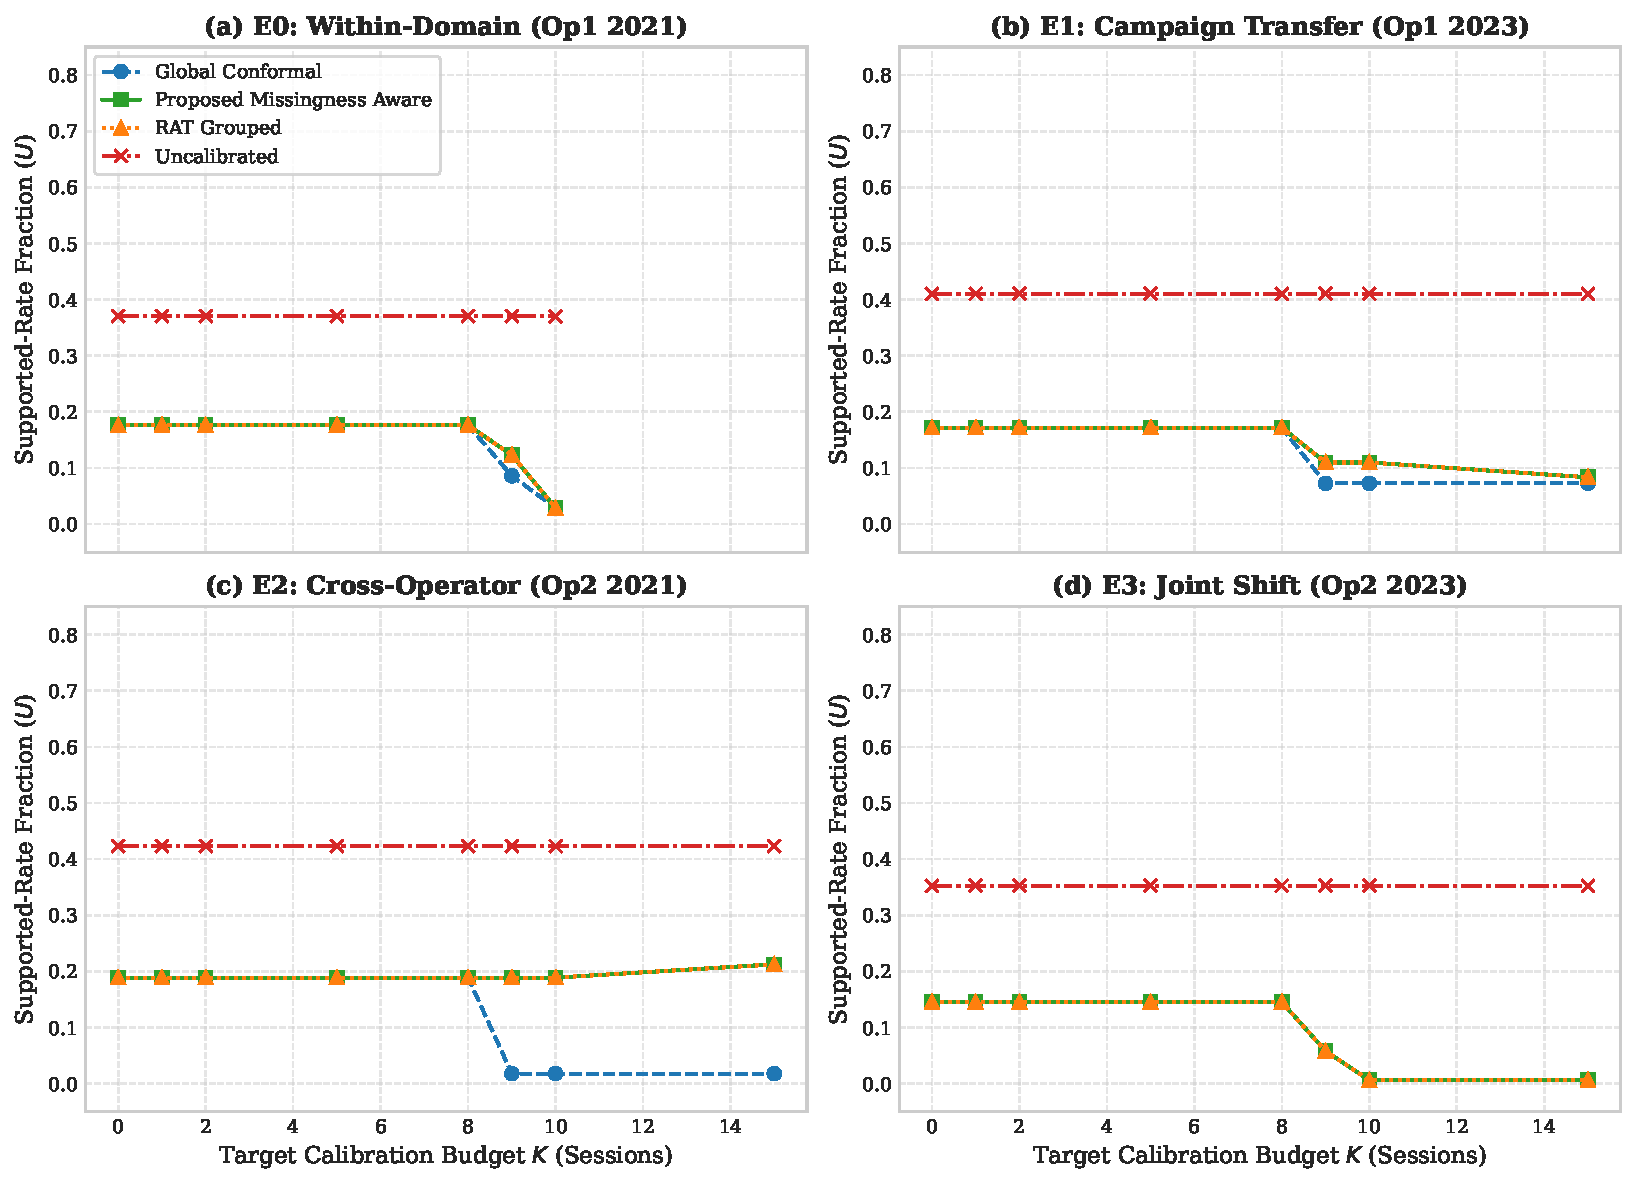
\includegraphics[width=.80\linewidth]{figures/fig1_budget_vs_usefulness.pdf}\caption{Performance across chronological calibration budgets. The same suffix is used at every available budget within a regime.}\end{figure}
\begin{figure}[!ht]\centering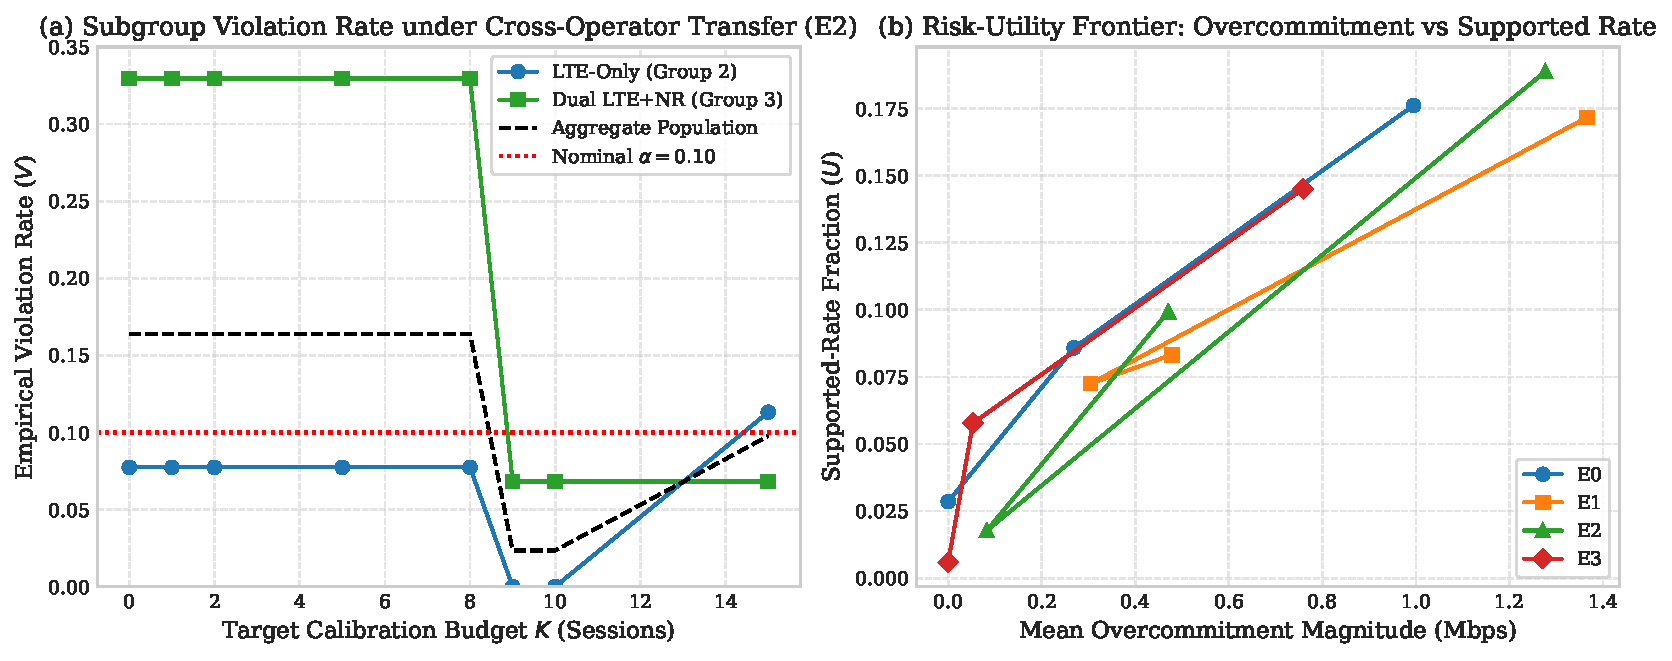
\includegraphics[width=.80\linewidth]{figures/fig2_subgroup_and_tradeoff.pdf}\caption{Subgroup performance and the empirical rate trade-off on the observed campaigns.}\end{figure}

\section{Sensitivity to the observational unit}
Table III compares the operational units. After numeric filtering, reset starts a segment on a drop exceeding 5 Mbps to below 5 Mbps. Relative drop starts on a drop exceeding 2 Mbps to below 1 Mbps. The active-start rule begins on an upward crossing above 1 Mbps or a gap over ten seconds. All three retain the last numeric row as the target. The active-start rule therefore frequently attaches the subsequent idle tail to the preceding burst. Its endpoint can differ even on a continuously logged trace. We use it as an alternative-endpoint stress test. There is no independent truth label for a physical download boundary. The reset rule aligns with a reinitializing mean-rate series and preserves the original benchmark definition. Its agreement with actual test starts remains unknown. The sensitivity analysis evaluates all eligible later pairs with a source-fitted model. Its denominator differs from the held-out benchmark. After excluding zero endpoints from scoring while keeping the fitted predictor, burst violations remain 0.3742 and 0.4651 on the two operators. Thus zero endpoints explain only part of the shift. Relative drop also changes the sample and the rates. None of these heuristics establishes ground-truth session boundaries.
\begin{table*}[!ht]
\centering\small
\caption{Source-only sensitivity across all eligible later-campaign pairs.}
\begin{tabular}{lrrrr}
\hline
Boundary & Segments & Zeros & E1V & E3V \\
Reset & 584 & 23 & 0.1479 & 0.2523 \\
Drop & 712 & 23 & 0.1339 & 0.2172 \\
Burst & 930 & 183 & 0.4024 & 0.4918 \\
\hline
\end{tabular}
\end{table*}

Median durations were 76, 72 and 53 seconds for reset, relative drop and active start. On later Op2 the corresponding tree errors were 27.41, 22.67 and 14.99 Mbps, while supported fractions were 0.2559, 0.2360 and 0.1490. A smaller absolute error coexisted with more violations as the endpoint population moved towards small values.

\section{Uncertainty and secondary experiments}
Table IV reports the paired contrasts. We resample collection dates with replacement, retaining all sessions from each selected date and pairing methods within each draw. The percentile endpoints from 2,000 draws describe empirical between-date variability conditional on this fitted model and prefix. Two to eight observed dates per regime offer little information about the population of future dates. A zero contrast interval follows algebraically when bounds coincide. Shared routes, equipment and measurement schedules can induce dependence across dates.
\begin{table*}[!ht]
\centering\small
\caption{Grouped minus global at ten sessions. Exploratory paired date bootstrap percentile endpoints.}
\begin{tabular}{lrrrrrrr}
\hline
Contrast & Days & dV & Vlo & Vhi & dU & Ulo & Uhi \\
E0D & 2 & 0.0000 & 0.0000 & 0.0000 & 0.0000 & 0.0000 & 0.0000 \\
E1D & 7 & 0.0000 & 0.0000 & 0.0000 & 0.0000 & 0.0000 & 0.0000 \\
E2D & 8 & 0.0000 & 0.0000 & 0.0000 & 0.0000 & 0.0000 & 0.0000 \\
E3D & 7 & 0.0000 & 0.0000 & 0.0000 & 0.0000 & 0.0000 & 0.0000 \\
\hline
\end{tabular}
\end{table*}

The repository includes every date's estimates and leave-one-date-out contrasts. Single-prefix testing leaves calibration-prefix variability unmeasured. Thirty-, sixty- and 120-second sensitivity runs change the eligible cohort and covariates together. Sixty seconds is the selected primary window. The supplementary analyses also examine group-support gates and artificial removal of observed NR fields. Artificial removal tests model response to controlled masking and does not identify why telemetry was absent in the field.

Table V and Figs. 3--5 report the feedback, weighting and decision analyses. The online experiment updates an offset after each observed label with a fixed step size. Its feedback requirements differ from static prefix calibration. This score-offset update is inspired by adaptive conformal inference \cite{gibbs2021adaptive}. The weighted experiment estimates source-to-target density ratios with a domain classifier and compares two clipping ranges. One variant uses calibration-pool covariates and the other uses unlabeled test covariates. The tight weight range is 0.1 to 10 and the wide range 0.01 to 100. Covariate-shift theory requires a stable conditional outcome law and appropriate density ratios \cite{tibshirani2019conformal}. Estimated, clipped weights and small effective sample sizes limit this interpretation. The alpha sweep and convex offline cost proxy show how the chosen threshold or penalty affects the displayed trade-off. The secondary sensitivity fits can use regime-specific source splits and should be compared within their own protocols.
\begin{figure}[!ht]\centering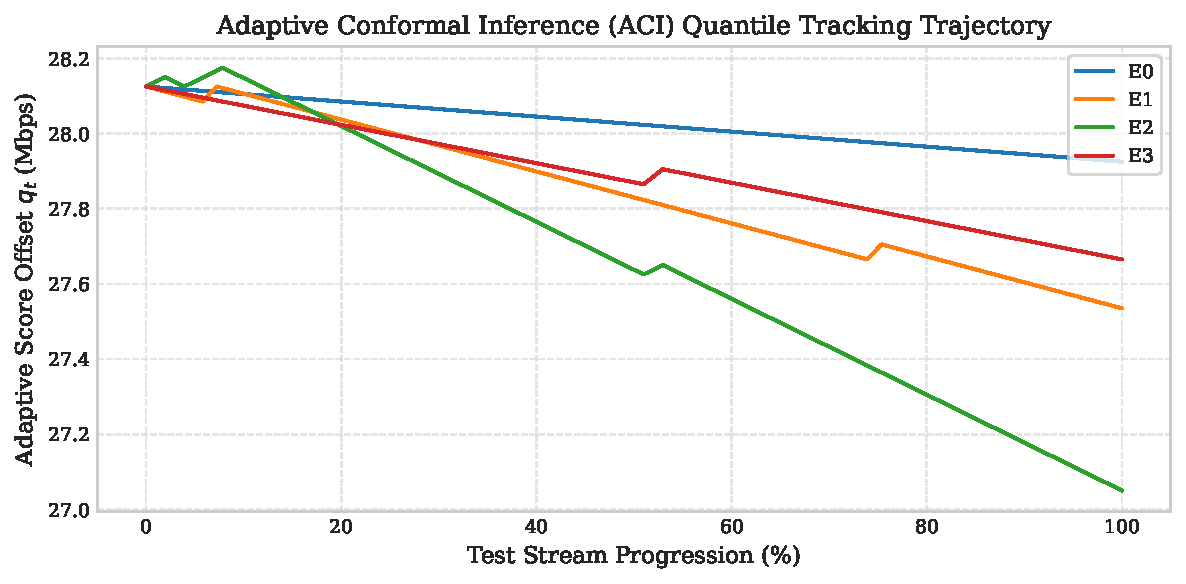
\includegraphics[width=.67\linewidth]{figures/fig3_aci_adaptation.pdf}\caption{Offset trajectory as labeled test sessions arrive in the online experiment.}\end{figure}
\begin{figure}[!ht]\centering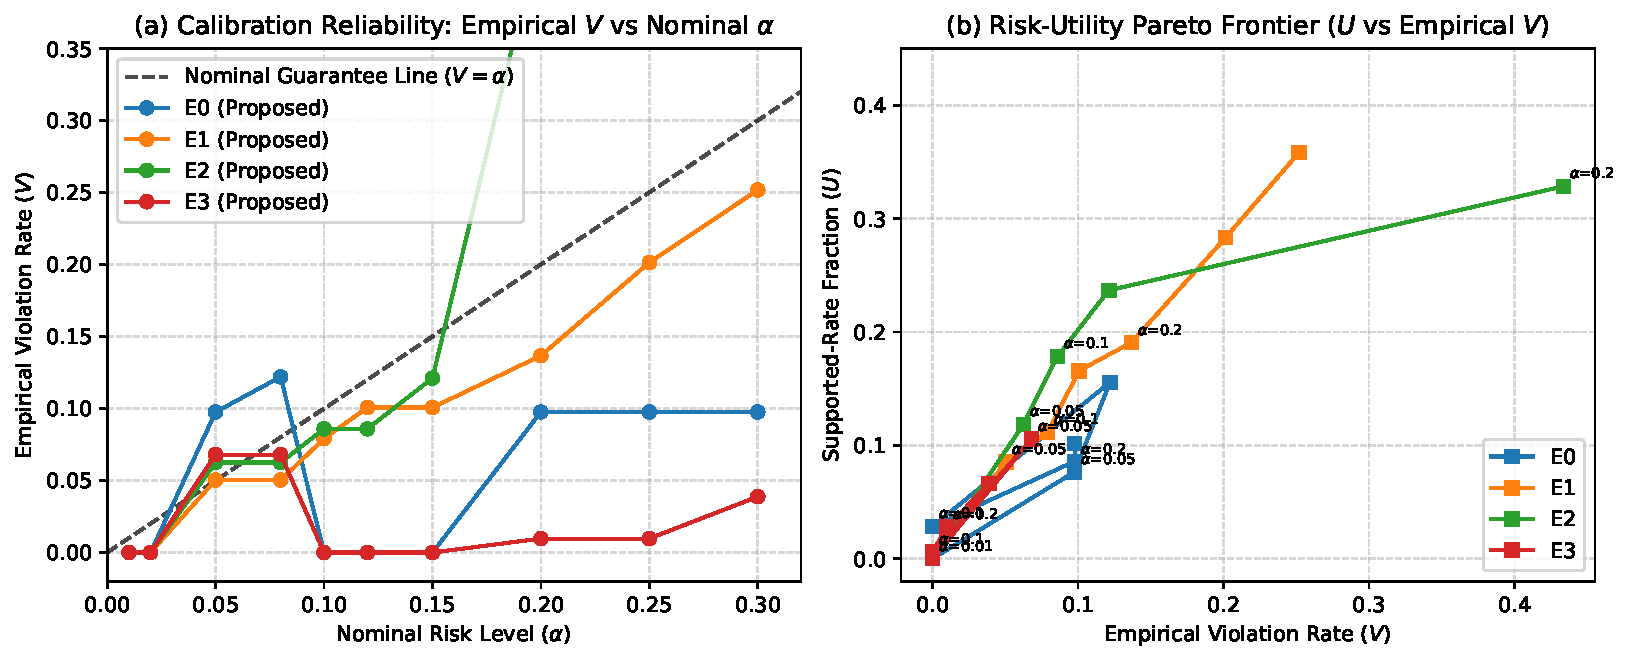
\includegraphics[width=.67\linewidth]{figures/fig4_pareto_frontier.pdf}\caption{Observed violations and supported throughput at the tested nominal levels.}\end{figure}
\begin{figure}[!ht]\centering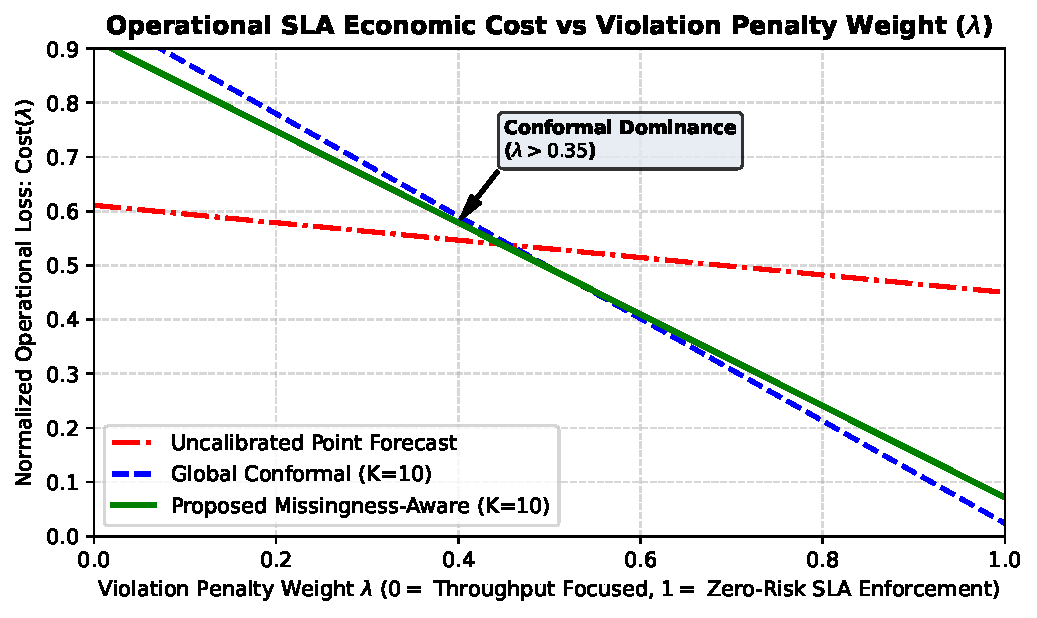
\includegraphics[width=.67\linewidth]{figures/fig5_sla_cost_curve.pdf}\caption{Offline loss under alternative weights on violations and unsupported throughput.}\end{figure}

\begin{table*}[!ht]
\centering\small
\caption{Online feedback and covariate weighting. A uses calibration-pool features and B uses test features. Tight and wide denote weight clipping ranges.}
\begin{tabular}{lrr}
\hline
Protocol & Violation & Supported \\
E0Online & 0.1220 & 0.1762 \\
E1Online & 0.1583 & 0.1653 \\
E2Online & 0.1562 & 0.1775 \\
E3Online & 0.1262 & 0.1447 \\
E1Atight & 0.0072 & 0.0127 \\
E1Awide & 0.0288 & 0.0450 \\
E1Btight & 0.0144 & 0.0063 \\
E1Bwide & 0.0000 & 0.0003 \\
E2Atight & 0.0156 & 0.0304 \\
E2Awide & 0.0156 & 0.0295 \\
E2Btight & 0.0469 & 0.0791 \\
E2Bwide & 0.0664 & 0.1130 \\
E3Atight & 0.0097 & 0.0159 \\
E3Awide & 0.0097 & 0.0083 \\
E3Btight & 0.0000 & 0.0096 \\
E3Bwide & 0.0000 & 0.0085 \\
\hline
\end{tabular}
\end{table*}

\section{External comparison and the value of a previous measurement}
We reproduced Sirhan's global one-sided forecast on the Irish 5G traces of Raca et al.\ \cite{sirhan2026handover,raca2020beyond}. Each of 30 splits assigns whole traces to training, calibration and testing. We retained the released features, predictor training and signed-error calibration. For target row $t+1$, persistence uses the downlink measurement at $t-1$, the latest throughput feature available to the tree. A second candidate takes the smaller of that lag and the nonnegative tree estimate before calibration. The Rome experiments informed the candidate choice before its Irish evaluation.

The published frontier chooses among twenty nominal levels using the realized test violations. Table VI averages the best supported fractions over feasible splits for each method. At ten percent, 29 splits were feasible for the global rule and all 30 for persistence and the minimum. The paired persistence gain was 3.58 percentage points on the 29 jointly feasible splits. The minimum lost 3.83 points on the corresponding comparison with global.
\begin{table*}[!ht]
\centering\small
\caption{Irish retrospective frontier. Budget and supported throughput are percentages. Gain is persistence minus rerun global in percentage points on jointly feasible splits. Wins counts positive paired gains.}
\begin{tabular}{lrrrrrr}
\hline
Budget & Published & Rerun & Minimum & Persistence & Gain & Wins \\
2 & 33.1 & 33.22 & 32.48 & 34.25 & 1.05 & 13/24 \\
5 & 47.2 & 47.14 & 45.27 & 49.73 & 2.58 & 22/28 \\
10 & 56.9 & 56.98 & 53.30 & 60.54 & 3.58 & 27/29 \\
\hline
\end{tabular}
\end{table*}


At a fixed nominal level of 0.10, all splits contribute. Persistence increased mean supported throughput from 55.60 to 59.44 percent and mean violations from 9.60 to 9.71 percent. Each rule met the ten percent target on 18 of 30 splits. The minimum reduced mean supported throughput to 52.81 percent.
\begin{table*}[!ht]
\centering\small
\caption{Irish fixed nominal ten percent. Mean violation and supported throughput are percentages. Passes counts splits meeting the target out of thirty.}
\begin{tabular}{lrrr}
\hline
Predictor & MeanV & MeanU & Passes \\
Global & 9.60 & 55.60 & 18 \\
Minimum & 9.72 & 52.81 & 17 \\
Persistence & 9.71 & 59.44 & 18 \\
\hline
\end{tabular}
\end{table*}


We kept each fitted forecast and calibration offset fixed and omitted traces only from test scoring. After dropping any one trace from every split in which it appeared, the mean paired gain ranged from 3.53 to 4.64 percentage points. Separately, we averaged each trace's utility difference over its test appearances. Persistence improved 79 of 83 traces, with a median gain of 5.04 points. The five largest download traces contributed 54.4 percent of the sum of measured rates across unique rows. Removing those traces raised the gain to 6.81 points. Removing all 21 download traces left 62 streaming traces and a gain of 10.96 points, alongside a higher violation rate than the tree. These sensitivity estimates reuse overlapping partitions of the same recordings.
\begin{table*}[!ht]
\centering\small
\caption{Irish fixed-setting exclusions from test scoring. Gain is the paired change in supported throughput in percentage points. Wins counts positive splits. Violation rates are percentages.}
\begin{tabular}{lrrrrr}
\hline
Sample & Omitted & Gain & Wins & TreeV & LagV \\
All & 0 & 3.84 & 27 & 9.60 & 9.71 \\
OmitTop5 & 5 & 6.81 & 29 & 5.89 & 7.14 \\
OmitDownloads & 21 & 10.96 & 30 & 2.90 & 4.86 \\
\hline
\end{tabular}
\end{table*}


Table IX compares recorded throughput transitions. NearZero counts endpoints at or below 0.001 Mbps. Fall and Rise count changes of at least 10 Mbps from the available lag in the indicated direction. NearZero can overlap Fall. A near-zero measurement does not identify an application stall. In Ireland the lag had a 6.59 Mbps mean absolute error. In the Rome joint shift (E3) it had a 35.44 Mbps error and 40.8 percent of endpoints fell at least 10 Mbps below the lag. On the first ten calibration sessions in E3, persistence supported 51.65 percent with 20.39 percent violations. The tree supported 0.60 percent with zero violations. With the same held-out suffix and eleven disjoint ten-label calibration blocks, persistence met the violation target zero times and the tree eleven times. The higher frequency of large downward changes is consistent with a riskier lag-based lower bound. Forecast horizon, endpoint construction, traffic mix and collection conditions differ together across the two datasets, so this comparison cannot isolate a cause.
\begin{table*}[!ht]
\centering\small
\caption{Lag versus endpoint on unique Irish rows and held-out Rome sessions. MAE is in Mbps. NearZero, Fall and Rise are percentages.}
\begin{tabular}{lrrrrrrr}
\hline
Setting & Pairs & Pearson & Spearman & LagMAE & NearZero & Fall & Rise \\
Ireland & 188545 & 0.77 & 0.67 & 6.59 & 45.0 & 5.8 & 6.3 \\
E0 & 41 & 0.29 & 0.41 & 35.14 & 0.0 & 22.0 & 22.0 \\
E1 & 139 & 0.52 & 0.57 & 32.69 & 7.2 & 37.4 & 14.4 \\
E2 & 256 & 0.70 & 0.61 & 17.57 & 2.0 & 19.1 & 16.0 \\
E3 & 103 & 0.49 & 0.55 & 35.44 & 1.0 & 40.8 & 24.3 \\
\hline
\end{tabular}
\end{table*}

\section{Outcome-independent scheduling and external evaluation}
In the later Rome release, a drop in measured throughput identifies both the start of a segment and the close of its predecessor. An observer who has yet to see that reading cannot identify the same candidate starts. To evaluate a trigger available at forecast time, we used each whole minute of logger operation and required a numeric rate in the preceding minute. Persistence predicts the last available reading in the next minute. We retained the original calendar partitions and calibrated on the first ten labeled opportunities. This changes the endpoint as well as the sample. Of 238 and 171 issued forecasts in E1 and E3, respectively, 211 and 152 had a target in a fully observed window. Missing labels could be informative.

Table X compares the two clock-triggered suffixes with an independent ten-label evaluation on Telenor HSDPA bus measurements released by Riiser et al.\ \cite{riiser2013commute}. We selected all logs on the first route listed by the publisher before measuring forecast performance. At each completed interval we predict the next interval's received bytes per elapsed second, converted to Mbps. Seven chronological dates supply three training dates, two calibration-pool dates and two test dates. The tree uses the last two rates; persistence uses the last rate. Both use the same ten target calibration labels. This evaluates the calibration procedure with a locally fitted predictor. The Irish results in Tables VI--VIII instead reproduce and extend an existing trace-level protocol. The Norwegian logs lack radio measurements needed to validate the grouped rule.
\begin{table*}[!ht]
\centering\small
\caption{Ten-label calibration for clock-triggered Rome forecasts and Norwegian interval forecasts. Error and offset are in Mbps. Violation and supported fractions are percentages.}
\begin{tabular}{lrrrrrrr}
\hline
Cohort & Model & Scored & Dates & MAE & Offset & Viol & Util \\
E1 & Persistence & 211 & 7 & 44.35 & 114.00 & 8.06 & 8.29 \\
E3 & Persistence & 152 & 7 & 50.72 & 53.90 & 13.82 & 16.00 \\
Norway & Persistence & 1278 & 2 & 0.38 & 1.49 & 0.78 & 26.78 \\
Norway & HistGBM & 1278 & 2 & 0.37 & 1.38 & 1.02 & 30.60 \\
\hline
\end{tabular}
\end{table*}

Figure 6 shows how often recalibration clips the commitment to zero at every available prefix length in the primary benchmark. This is the fraction of opportunities on which a lower forecast makes no positive rate commitment.
\begin{figure}[!ht]\centering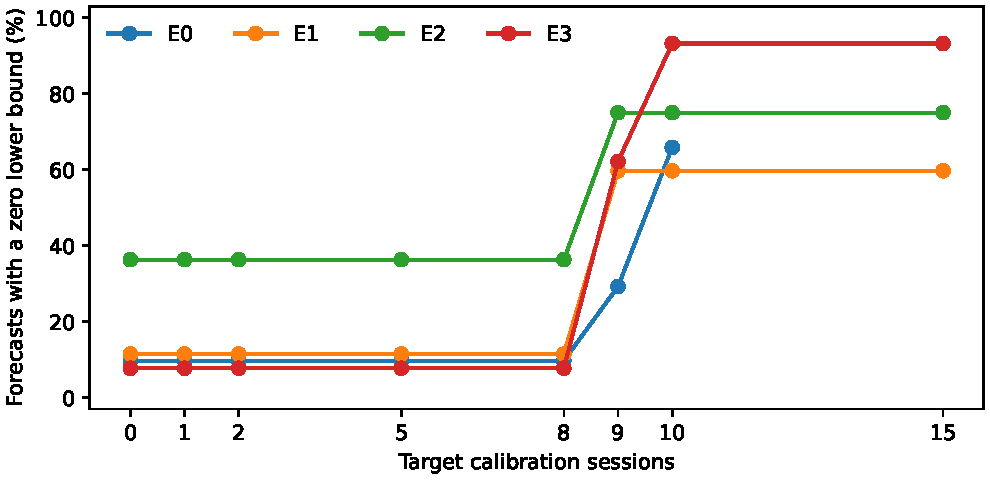
\includegraphics[width=.67\linewidth]{figures/fig6_zero_bounds.pdf}\caption{Fraction of zero global lower bounds by target calibration budget and Rome regime.}\end{figure}

For reset-based persistence in Rome E3, violations and supported throughput were 20.39 and 51.65 percent. With the clock they were 13.82 and 16.00 percent. On the Norwegian route both methods met the empirical violation target on the pooled suffix. Their two test dates provide little information about other days or routes. Neither experiment measures prospective application outcomes.
Finally we applied the missingness rule to the Irish measurements in a separate chronological analysis (Table XI). We used the current availability of numeric primary and NR signal-power fields before any forward filling, the preceding downlink as the point forecast, and the following row as the endpoint. We required strictly ordered lag, issue and target timestamps. The first eleven of 27 collection dates supplied the calibration pool. On the remaining sixteen dates, point MAE was 9.05 Mbps. All first ten calibration rows lacked an NR reading, so both rules gave the same bound on all 108,519 test rows. Violations reached 34.81 percent. Deleting one test date at a time gave 34.03 to 36.68 percent. Even with all 64,265 calibration rows, grouped violations remained 29.86 percent. This failure on a chronological split limits the interpretation of the favorable random-trace results. Split, calibration size and timestamp eligibility differ together.
\begin{table*}[!ht]
\centering\small
\caption{Chronological Irish persistence forecasts on 108519 rows from sixteen suffix dates. Local counts forecasts using a group-specific offset. Performance measures are percentages.}
\begin{tabular}{lrrrrr}
\hline
Labels & Rule & Local & Coverage & Violation & Supported \\
10 & Global & 0 & 65.19 & 34.81 & 71.62 \\
10 & Grouped & 21372 & 65.19 & 34.81 & 71.62 \\
64265 & Global & 0 & 69.50 & 30.50 & 71.31 \\
64265 & Grouped & 108519 & 70.14 & 29.86 & 71.36 \\
\hline
\end{tabular}
\end{table*}

\section{Conclusion}
A short prefix produced conservative lower forecasts in these traces, sometimes at the cost of nearly all usable throughput. The first finite target rank at nine labels is specific to the chosen nominal level. The burst-endpoint diagnostic and sparse calendar-day support limit generalization. More independent measurement dates and a logger that records physical test starts before throughput is observed would allow the session forecast to be evaluated prospectively.
\section*{Acknowledgment}
OpenAI Codex assisted with code development, experimental checks and drafting and revising the manuscript.
\bibliographystyle{IEEEtran}
\bibliography{references}
\end{document}
